% !TEX TS-program = pdflatex
\documentclass[aps,prc,twocolumn,floatfix,showpacs,preprintnumbers,amsmath,amssymb,superscriptaddress,linenumbers]{revtex4-1}
\usepackage{hyperref}
\usepackage{latexsym}
\usepackage{verbatim}
\usepackage{graphics}
\usepackage{caption}
\usepackage{subfigure}
\usepackage{amsmath}
\captionsetup{justification=centerlast,font=small,margin=0.5cm}
\usepackage{setspace}
\usepackage{graphicx,amsmath,color}% Include figure files
\usepackage[normalem]{ulem} %for strikeouts
\usepackage{todonotes}
\usepackage{placeins}


\providecommand{\Journal}[4] {#1 {\bf #2}, #3 (#4)}
\providecommand{\EPJC}{Eur. Phys. J. C }
\providecommand{\NCA}{Nuovo Cimento }
\providecommand{\NIM}{Nucl. Instr. Methods }
\providecommand{\NIMA}{Nucl. Instr. Meth. A }
\providecommand{\NPA}{Nucl. Phys. A }
\providecommand{\NPB}{Nucl. Phys. B }
\providecommand{\NHPA}{Nucl. Hadr. Phys. A }
\providecommand{\PLB}{Phys. Lett. B }
\providecommand{\PR}{Phys. Rev. }
\providecommand{\PRL}{Phys. Rev. Lett. }
\providecommand{\PRC}{Phys. Rev. C }
\providecommand{\PRD}{Phys. Rev. D }
\providecommand{\RMP}{Rev. Mod. Phys. }
\providecommand{\ZPC}{Z. Phys. C }
\providecommand{\qqb}{$q\bar{q}$~}
\newcommand{\bff}{{}}

\definecolor{lightred}{rgb}{1,0.5,0.5}
\definecolor{lightgreen}{rgb}{0.5,1,0.5}
\definecolor{darkgreen}{rgb}{0.5,0.9,0.5}

\def\piz{\pi^{0}}
\def\pizT{$\pi^{0} \ $}
\def\epemT{$ e^+e^-  $}
\def\epem{e^+e^-}

\definecolor{Mycolor2}{HTML}{0c9008}

\begin{document}
\preprint{}

\title{Photoproduction of $\pi^0$ on Hydrogen using \epemT($\gamma$) detection mode with CLAS}

%To be submitted to Phys. Rev. Lett.\\
%\bf -- DRAFT -- VERSION 21\\
%\bf \today}

\newcommand*{\ODU}{Old Dominion University, Norfolk, VA 23529, USA}
\newcommand*{\IKP}{Institut f\"ur Kernphysik, Forschungszentrum J\"ulich, 
	52424 J\"ulich, Germany}
\newcommand*{\BOCHUM}{Institut f\"ur Experimentalphysik I, Ruhr-–Universit\"at 
	Bochum, 44780 Bochum, Germany}
\newcommand*{\JARA}{ JARA–FAME, J\"ulich Aachen Research Alliance, 
	Forschungszentrum J\"ulich, 52425 J\"ulich, and RWTH Aachen, 52056 
	Aachen, Germany}
\newcommand*{\KYUNGPOOK} {Kyungpook National University, 702-701, Daegu, 
	Republic of Korea}
\newcommand*{\INR}{Institute for Nuclear Research, 117312, Moscow, Russia}
\newcommand*{\CUA}{Catholic University of America, Washington, DC 20064} 
\newcommand*{\JLAB}{Thomas Jefferson National Accelerator Facility, Newport 
	News, VA 23606}
\newcommand*{\UVA}{University of Virginia, Charlottesville, VA 22904, USA}
\newcommand*{\CMU}{Carnegie Mellon University, Pittsburg, PA 15213, USA}

\newcommand*{\ANL}{Argonne National Laboratory, Argonne, IL 60439, USA}
\newcommand*{\ASU}{Arizona State University, Tempe, AZ 85287, USA}
\newcommand*{\CSUDH}{California State University, Dominguez Hills, Carson, 
	CA 90747, USA}
\newcommand*{\CANISIUS}{Canisius College, Buffalo, NY, USA}
\newcommand*{\SACLAY}{CEA, Centre de Saclay, Irfu/Service de Physique 
	Nucl\'eaire, 91191 Gif-sur-Yvette, France}
\newcommand*{\CNU}{Christopher Newport University, Newport News, VA 23606, 
	USA}
\newcommand*{\UCONN}{University of Connecticut, Storrs, CO 06269, USA}
\newcommand*{\EDINBURGH}{University of Edinburgh, Edinburgh EH9 3JZ, United 
	Kingdom}
\newcommand*{\FU}{Fairfield University, Fairfield, CT 06824, USA}
\newcommand*{\FIU}{Florida International University, Miami, FL 33199, USA}
\newcommand*{\FSU}{Florida State University, Tallahassee, FL 32306, USA}
\newcommand*{\GWU}{The George Washington University, Washington, DC 20052, USA}
\newcommand*{\ISU}{Idaho State University, Pocatello, Idaho 83209, USA}
\newcommand*{\INFNFE}{INFN, Sezione di Ferrara, 44100 Ferrara, Italy}
\newcommand*{\INFNFR}{INFN, Laboratori Nazionali di Frascati, 00044 Frascati, 
	Italy}
\newcommand*{\INFNGE}{INFN, Sezione di Genova, 16146 Genova, Italy}
\newcommand*{\INFNRO}{INFN, Sezione di Roma Tor Vergata, 00133 Rome, Italy}
\newcommand*{\ORSAY}{Institut de Physique Nucl\'eaire ORSAY, Orsay, France}
\newcommand*{\ITEP}{Institute of Theoretical and Experimental Physics, Moscow, 
	117259, Russia}
\newcommand*{\JMU}{James Madison University, Harrisonburg, VA 22807, USA}
\newcommand*{\KNU}{Kyungpook National University, Daegu 702-701, Republic of 
	Korea}
\newcommand*{\LPSC}{LPSC, Universite Joseph Fourier, CNRS/IN2P3, INPG, 
	Grenoble, France}
\newcommand*{\UNH}{University of New Hampshire, Durham, New Hampshire 03824, 
	USA}
\newcommand*{\NSU}{Norfolk State University, Norfolk, VA 23504, USA}
\newcommand*{\OHIOU}{Ohio University, Athens, Ohio  45701, USA}
\newcommand*{\RPI}{Rensselaer Polytechnic Institute, Troy, NY 12180, USA}
\newcommand*{\ROMAII}{Universita' di Roma Tor Vergata, 00133 Rome Italy}
\newcommand*{\MSU}{Skobeltsyn Nuclear Physics Institute, 119899 Moscow, Russia}
\newcommand*{\SCAROLINA}{University of South Carolina, Columbia, South Carolina 
	29208, USA}
\newcommand*{\UNIONC}{Union College, Schenectady, NY 12308}
\newcommand*{\UTFSM}{Universidad T\'{e}cnica Federico Santa Mar\'{i}a, Casilla 
	110-V Valpara\'{i}so, Chile}
\newcommand*{\GLASGOW}{University of Glasgow, Glasgow G12 8QQ, United Kingdom}
\newcommand*{\VIRGINIA}{University of Virginia, Charlottesville, VA 22901, 
	USA}
\newcommand*{\WM}{College of William and Mary, Williamsburg, VA 23187, USA}
\newcommand*{\YEREVAN}{Yerevan Physics Institute, 375036 Yerevan, Armenia}
\newcommand*{\NOWCNU}{Christopher Newport University, Newport News, VA
	23606, USA}
\newcommand*{\NOWLANL}{Los Alamos National Laboratory, Los Alamos, NM 87544, 
	USA}
\newcommand*{\NOWMSU}{Skobeltsyn Nuclear Physics Institute, 119899 Moscow, 
	Russia}
\newcommand*{\NOWORSAY}{Institut de Physique Nucl\'eaire ORSAY, Orsay, France}
\newcommand*{\TUFTS}{Tufts University, Medford, MA 02155, USA}
%%%%%%%%% END OF Latex Macros for institute addresses  %%%%%%%%%%%%%%%%%%

\author {Michael~C.~Kunkel}
%\altaffiliation[Now at the ]{Institut f\"ur Kernphysik, Forschungszentrum 
%	J\"ulich, 52424 J\"ulich, Germany}%Lines break automatically or can be forced with \\
\affiliation{\ODU}
\affiliation{\IKP}
\author {Moskov~J.~Amaryan}
\thanks{Corresponding author; mamaryan@odu.edu}
%\email{mamaryan@odu.edu}
\affiliation{\ODU}
\author {Igor~I.~Strakovsky}
\affiliation{\GWU}
\author {James~Ritman}
\affiliation{\IKP}
\affiliation{\BOCHUM}
\author{Gary~R.~Goldstein}
\affiliation{\TUFTS}
%%%%%%%%%%%%%%%%%%%%%%%%%%%%%%%%%%%%%%%%%%%%%%%%%%%%%%%%%%%%%%%%%%%%%%%%%%%%
%
\vskip 1.50in
\vskip 2in

%---------------------------------------------
\begin{abstract}
\centerline{\Large Abstract}
\vskip 0.2in
We report the first high precision measurement of the exclusive $\pi^0$ 
photoproduction cross section via Dalitz decay and $e^+e^-$ pair conversion 
mode on a hydrogen target in a wide kinematic range with the CLAS setup at 
Thomas Jefferson National Accelerator Facility. The measurement was performed using data from the reaction 
$\gamma p\rightarrow pe^+e^-X(\gamma)$ using a 
tagged photon beam spanning an energy interval from the ``resonance'' to 
the ``Regge'' regimes, i.e photon energies $E = 1.25-5.55$~GeV. The final 
state particles $p;e^+;e^-$ were detected \textcolor{red}{whereas} the photon was 
inferred from energy and momentum conservation. This new data sample quadrupled the \textcolor{red}{world database for $\pi^{0}$ photoproduction}
above E = 2~GeV. Our data appear to favor the Regge pole model and the 
constituent counting rule while disfavoring the Handbag 
model.
\end{abstract}
%---------------------------------------------

\pacs{12.38.Aw, 13.60.Rj, 14.20.-c, 25.20.Lj}
\maketitle

%---------------------------------------------
%\textbf{Introduction:} 

The rich pion-nucleon resonance spectrum for center-of-mass 
(c.m.) energies up to 2.5~GeV provides insights and challenges concerning 
the workings of the strong interaction through partial wave expansions, 
exchange potentials, non-relativistic quark models and QCD. Photoproduction of $\pi^0$ and $\eta$ mesons has always enabled complementary investigations, constrained various models, and led to further insights. At the interface between the crowded low energy resonance 
production and the smooth higher energy, small angle behavior, 
traditionally described by Regge poles~\cite{Ader:1967tqj}, lies a 
region in which hadronic duality interpolates the different excitation function
behavior. Exclusive $\pi$ photoproduction and $\pi$ nucleon elastic 
scattering show this duality in a semi-local sense through Finite Energy 
Sum Rules (FESR)~\cite{Armenian:1974xd}. The connection to QCD is more 
tenuous for on-shell photoproduction of pions at small scattering angles, 
but the quark content can become manifest through large fixed angle 
dimensional counting rules~\cite{Brodsky:1973kr} as well as being evident 
in semi-inclusive or exclusive electroproduction of pions, described 
through Transverse Momentum Distributions (TMDs)  and Generalized Parton 
Distributions (GPDs).

%---------------------------------------------------
%\textbf{Regge Pole Model:} 

The Regge pole description of photoproduction amplitudes 
has a long and varied history. For $\pi^0$ and $\eta$ photoproduction, 
all applications rely on a set of known meson Regge poles. There are 
two allowed t-channel J$^{PC}$ quantum numbers, the odd-signature (odd spin) 
1$^{--}$ ($\rho^0$, $\omega$) and the 1$^{+-}$ ($b^0_1$, $h_1$) Reggeons. Regge cut amplitudes are 
incorporated into some models and are interpreted as rescattering of 
on-shell meson-nucleon amplitudes.  The phases between the different 
poles and cuts can be critical in determining the polarizations and the 
constructive or destructive interferences that can appear. Four distinct Regge models 
are considered here.

The oldest model developed by Goldstein and 
Owens~\cite{Goldstein:1973xn} has the exchange of leading Regge 
trajectories with appropriate t-channel quantum numbers along with 
Regge cuts generated via final state rescattering through Pomeron 
exchange. The Regge couplings to the nucleon were fixed by reference 
to electromagnetic form factors, SU(3)$_{flavor}$, and low energy 
nucleon-nucleon meson exchange potentials. At the time, the range of 
applicability was taken to be above the resonance region and $\mid 
t \mid \le 1.2 \, {\rm GeV}^2$, where $t$ is the squared 
four-momentum transfer. Here we will let the $\mid t \mid$ 
range extend to large $\mid t \mid$ in order to see the predicted cross 
section dips from the zeroes in Regge residues. Because even signature partners ($A_2$, etc.) of the odd spin poles ($\rho$, etc.) lie on the same trajectories, the Regge residues are required to have zeroes to cancel the even (wrong) signature poles in the physical region - “nonsense wrong signature zeroes (NWSZ). While the dip near 
$t\approx -0.5$ GeV$^2$ is present in $\pi^0$ data, it is not in the 
recent beam asymmetry data on $\eta$ 
photoproduction~\cite{AlGhoul:2017nbp}. This is not explained by the 
standard form of the NWSZ Regge residues. 
  
Quite recently, Mathieu {\it et al.}~\cite{Mathieu:2015eia} (JPAC) 
(see also~\cite{Kashevarov:2017vyl}), used the same set of Regge poles, 
but a simplified form of only $\omega$ -Pomeron cuts. They show that 
daughter trajectories are not significant as an alternative to the 
Regge cuts. However, to explain the lack of $t\approx -0.5$ GeV$^2$ 
dip in $\eta$ photoproduction, they remove the standard wrong signature 
zero, {\it ad hoc}.  Donnachie and Kalashnikova~\cite{Donnachie:2015jaa} 
have included t-channel $\rho^0$, $\omega$, and the $b^0_1$, but not 
the $h_1$ Reggeon, all with different parameterizations from 
Ref.~\cite{Goldstein:1973xn}. They include $\omega, \rho \times {\rm 
Pomeron}$ cuts, as well as $\omega, \rho \times {\rm f}_2$ lower lying 
cuts, which help to fill in the wrong signature zeroes of the $\omega, 
\rho$ Regge pole residues. The model of Laget and 
collaborators~\cite{Laget:2005be} included u-channel baryon exchange. 
That model also connected the small and large t-channel regimes by a 
mechanism called ``saturating" the Regge trajectories at $\alpha(t) \, 
\rightarrow \, -1$ for $t < -1.5$ GeV$^2$, thereby describing the full 
angular range ($\theta = 0 - 2\pi$), while the other models are good 
for more limited ranges of $t$~\cite{Goldstein:1973xn,Mathieu:2015eia,
Donnachie:2015jaa}. Here, we examine how Regge phenomenology works for 
the energy range of 2.8~GeV $< $ E$_\gamma$ $<$ 5.5~GeV.

%--------------------------------------------------
%\textbf{Handbag Model:}
 
In addition to Regge pole models, the introduction of the handbag mechanism, developed by 
Kroll \textit{et al.}~\cite{Huang:2000kd}, has provided complimentary 
possibilities for the interpretation of hard exclusive reactions. In 
this approach, the reaction is factorized into two parts, one quark 
from the incoming and one from the outgoing nucleon participate in the 
hard sub-process, which is calculable using pQCD. The soft part 
consists of all the other partons that are spectators and can be 
described in terms of GPDs~\cite{Ji:1996nm}.
The HERMES measurement of beam asymmetry in DVCS was the first 
to confirm the azimuthal dependence expected from the GPD interpretation~\cite{Amarian:2000vx}.
The handbag model applicability requires a hard scale, which, for meson 
photoproduction, is only provided by large transverse momentum. That 
corresponds to large angle production, roughly for 
$-0.6~\leq\cos\theta~\leq 0.6$.  Here, we examined how the handbag 
model may extend for the $\gamma p\rightarrow p\pi^0$ case as Kroll 
\textit{et al.} proposed. The distribution amplitude for the 
quark+antiquark to $\pi^0$ is fixed by other phenomenology and 
leads to the strong suppression of the productions cross section.	


%--------------------------------------------------
%\textbf{Scaling:} 

Binary reactions in QCD, with large momentum transfer 
occur via gluon and quark exchanges between colliding particles. The 
constituent counting rules of Brodsky and Farrar~\cite{Brodsky:1973kr} 
has a simple recipe to predict the energy dependence of the 
differential cross sections of two-body reactions at large angles 
when $t/s$ is finite and is kept constant.  The lightest meson 
photoproduction was examined in terms of the counting 
rules~\cite{Anderson:1976ph,Jenkins:1995bk,Zhu:2002su,Chen:2009sda,
Kong:2015yzn}. As has been observed, first of all at SLAC by 
Anderson \textit{et al.}, the reaction $\gamma p\rightarrow\pi^+n$ 
shows agreement with constituent counting rules that predict the 
cross section should vary as $s^{-7}$~\cite{Anderson:1976ph}. The 
agreement extends down to s = 6~GeV$^2$ where baryon resonances are 
still playing a role.  Here, we examined how applicable the counting rule is 
for $\gamma p\rightarrow\pi^0p$ up to s = 10~GeV$^2$. 

Previous bremsstrahlung measurements of $\gamma p\rightarrow p\pi^0$, for $2~\leq E\leq 
18$~GeV (1964 -- 1979) provided 451 data points of $d\sigma/dt(|t|)$s~\cite{brem}, have very large systematic 
uncertainties and do not have sufficient accuracy to perform 
comprehensive phenomenological analyses.  A previous CLAS measurement of $\gamma p\rightarrow p\pi^0$, for $2.0~\leq E\leq 2.9$~GeV has an overall systematic uncertainty of 5\% but only provided 164 data points of $d\sigma/dt(|t|)$s~\cite{Dugger:2007bt}.

The results described here are the first to allow a detailed analysis, bridging the nucleon resonance and high energy regions over a wide angular range, of exclusive pion photoproduction. By significantly extending the database they facilitate
the examination
%The new measurement, presented here, currently is the only 
%		measurement that bridges resonance and high energy, both narrow and wide 
%		angles, regions of exclusive $\pi^0$ photoproduction. This significantly 
%		extends the available database, facilitating the examination 
%		 
		of the resonance, ``Regge", and wide angle QCD regimes of phenomenology. The 
		broad range of c.m. energy, $\sqrt{s}$, is particularly helpful in 
		sorting out the phenomenology associated with both Regge and QCD-based 
		models of the nucleon~\cite{Kroll:2017hym}.

In this work, we provide a large set of differential 
cross section values from $E$ = 1.275 to 5.425~MeV in laboratory photon 
energy, corresponding to a range of c.m. energies, $W$ = 1.81 -- 
3.33~GeV.  We have compared the Regge pole, the handbag, and the 
constituent counting rule phenomenology with the new CLAS experimental 
information on $d\sigma/dt(|t|)$ for the $\gamma p\rightarrow\pi^0p$ 
reaction above the ``resonance" regime. As will be seen, this data 
set quadruples the world bremsstrahlung database above E = 2~GeV and 
constrains the high energy phenomenology well with a previous CLAS 
measurement~\cite{Dugger:2007bt}.

%------------------------------------------------------------------
%\textbf{Experiment:} 

The experiment was performed during March-June, 2008
with the CLAS setup at TJNAF using a tagged photon beam produced by 
bremsstrahlung from the 5.72~GeV electron beam provided by the CEBAF 
accelerator, which impinged upon a liquid hydrogen target,
%. 
%The experiment as a whole was a set of different 
%experiments running at the same time with the same experimental 
%configuration (cryogenic target, tagger, trigger configuration, and CLAS) 
and was designated with the name ``g12". 
The experimental details are given in Ref.~\cite{g12}. The reaction 
of interest is the photoproduction of neutral pions on a hydrogen 
target $\gamma p\rightarrow p\pi^0$, 
where the neutral pions decay into a $e^+e^-\gamma$ final state either due to external conversion, $\pi^0 \rightarrow\gamma\gamma 
\rightarrow e^+e^-\gamma$ or via Dalitz decay $\pi^0
\rightarrow\gamma^\ast\gamma\rightarrow e^+e^-\gamma$. Running the 
experiment at high beam current was possible due to the final state 
containing three charged tracks, $p;e^+;e^-$, as opposed to single 
prong charged track detection, which impose limitations due to trigger 
and data acquisition restrictions.

%----------------------------------------------------------
%\textbf{Data analysis:} 

Particle identification for the experiment was based on $\beta$ vs. momentum$\times$charge. 
Lepton identification was based on a kinematic constraint to the $\pi^0$ mass. 
Once the data was skimmed for p, $\pi^+$, $\pi^-$, 
all particles that were $\pi^+$, $\pi^-$ were tentatively assigned 
to be electrons or positrons based on their charge (for details, 
see Ref.~\cite{Kunkel}). After particle selection, standard $g12$ 
calibration, fiducial cuts~\cite{g12} and timing cuts were applied 
in the analysis.
%-------------------------------------------------------
\begin{figure*}[htb!]
        \centerline{
               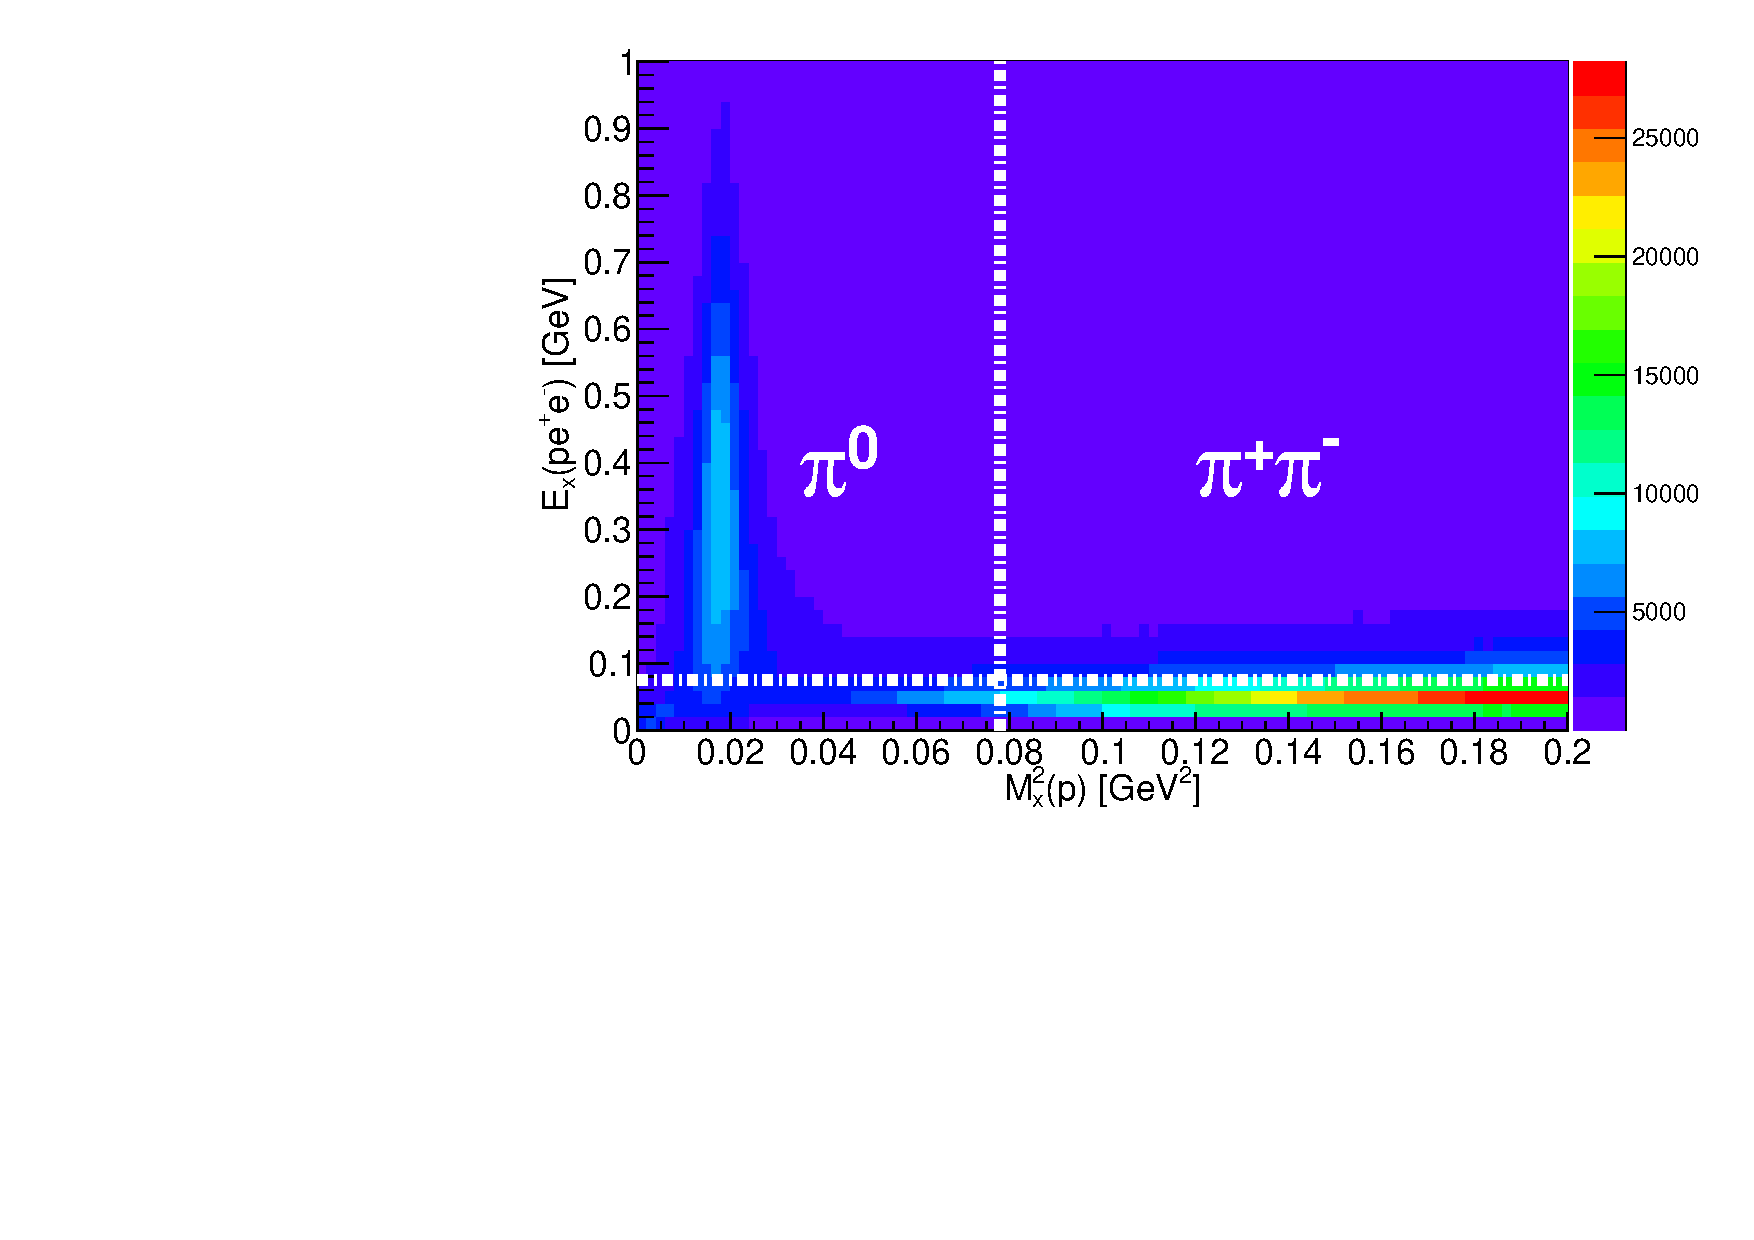
\includegraphics[height=0.35\textwidth,width=0.5\textwidth]{ME_vs_mxpcompare.pdf}\hfill
               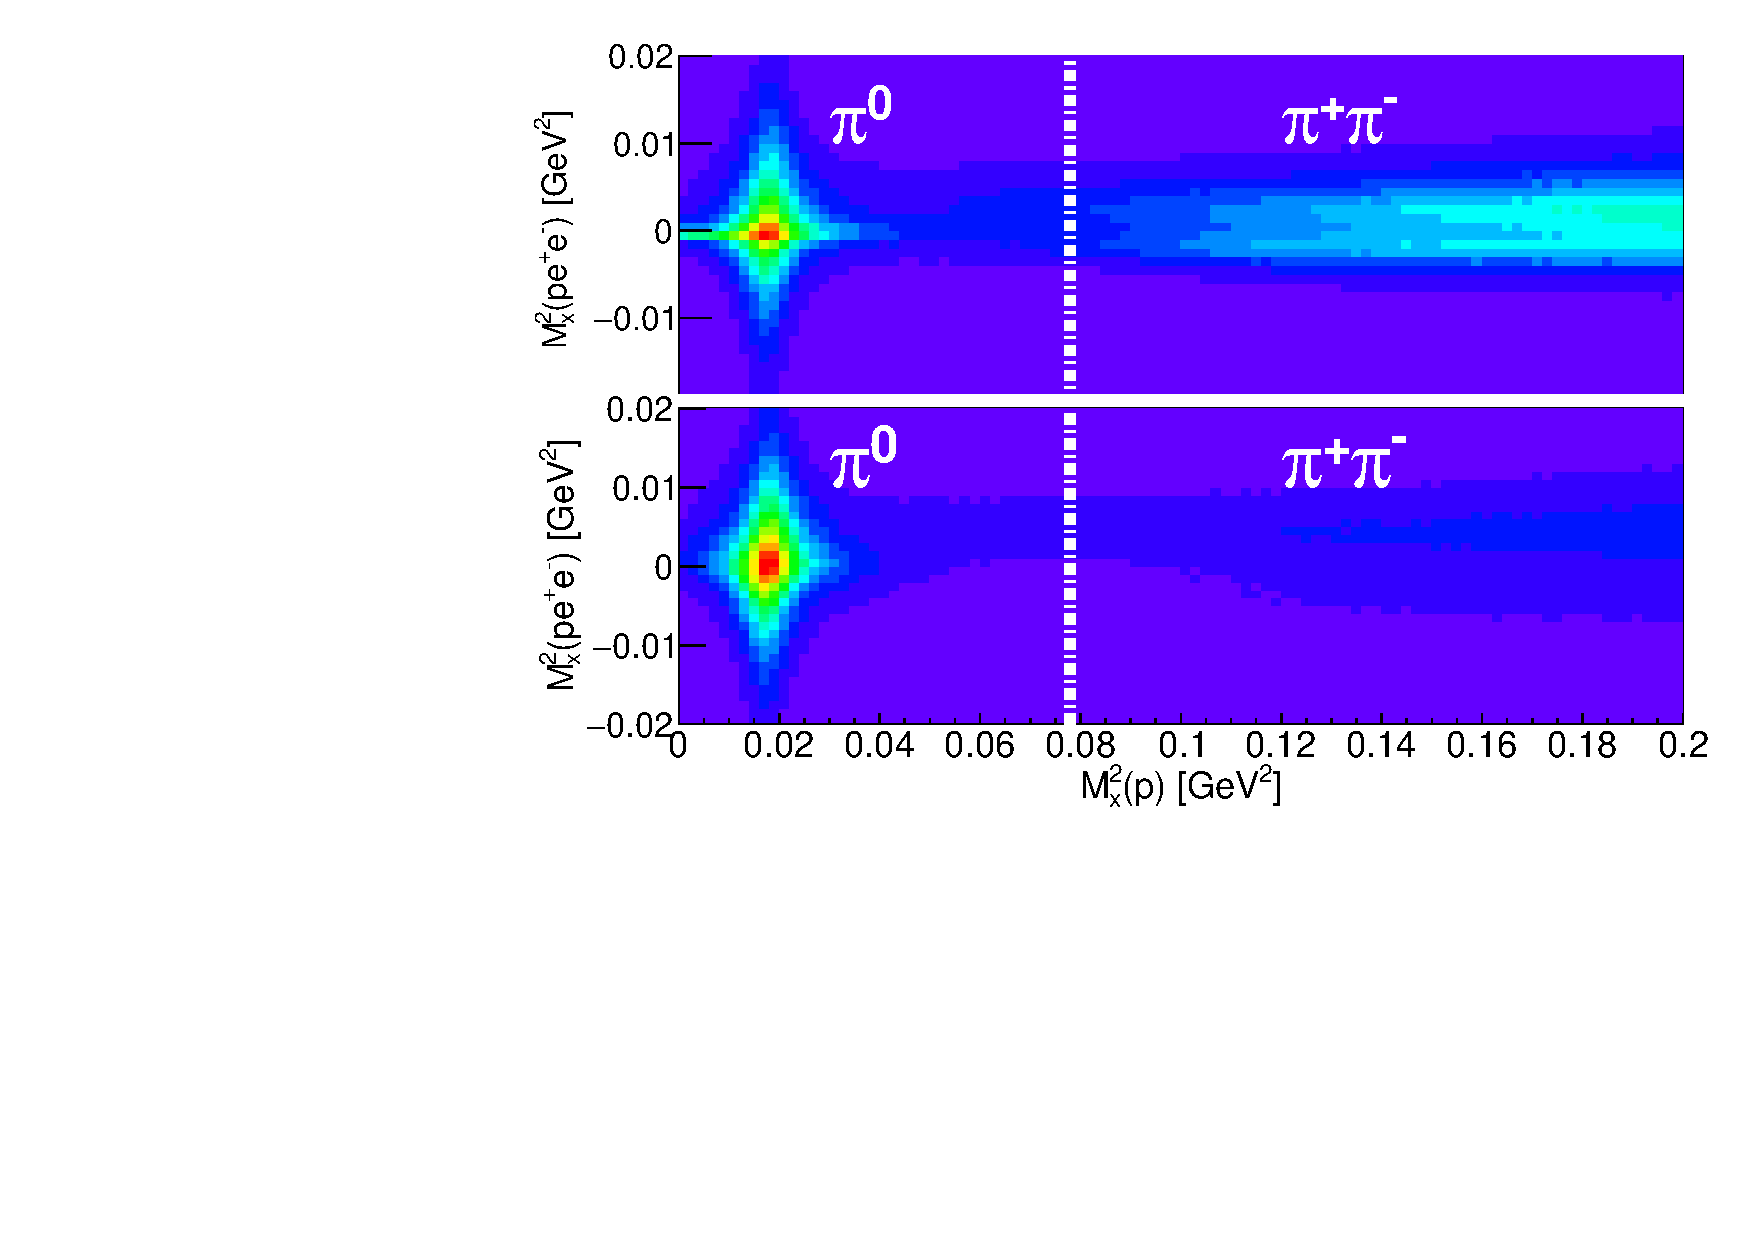
\includegraphics[height=0.35\textwidth,width=0.5\textwidth]{mm2_vs_mxp_compare.pdf}}

        \caption{(Color online)(left panel)Missing energy $\mathrm{M_E(pe^+e^-)}$ of all detected particles vs missing mass squared of the proton $  \mathrm{M_x^2(p)}$. (Right panel) Missing mass squared of all detected particles $\mathrm{M_x^2(pe^+e^-)}$ vs 
        	missing mass of the proton $\mathrm{M_x^2(p)}$; (right-top panel) before applying the
        	$\mathrm{M_E(pe^+e^-)} <$ 75~MeV condition, (right-bottom panel)
        	after applying the $\mathrm{M_E(pe^+e^-)} >$ 75~MeV condition.
        	The horizontal white dashed-dotted line depicted on the left
        	panel illustrates the 75~MeV threshold used in this analysis.
        	The vertical white dashed-dotted line depicts the kinematic
        	threshold for $\pi^+\pi^-$ production.}
        \label{fig:sys}
\end{figure*}

Different kinematic fits were employed to cleanly identify the 
$\gamma p\rightarrow pe^+e^-(\gamma)$ reaction. They were applied 
to filter background from misidentified double pion production to 
the single $\pi^0$ production, to constrain the missing mass of entire 
final state to a missing photon and to ensure that the fit to the missing 
photon constrained the squared invariant 
mass of $e^+e^-(\gamma)$=m$^2_{\pi^0}$. The values of the confidence levels cuts employed was 
determined using statistical significance to get the best signal/background ratio.

%The analysis employed three separate kinematic fitting 
%hypotheses, 4-C, 1-C, and 2-C, as well as a cut on the missing 
%energy of the detected system. The 4-C fit used the $\gamma 
%p\rightarrow p\pi^+\pi^-$ channel to filter background from double 
%charged pion production from single $\pi^0$ production. The 1-C fit
%was used for the topology of $\gamma p\rightarrow pe^+e^-(\gamma)$ 
%to fit to a missing final state photon.  The 2-C fit was used for 
%the topology of $\gamma p\rightarrow pe^+e^-(\gamma)$ to fit to a 
%missing final state photon but also to constrain the squared invariant 
%mass of $e^+e^-(\gamma)$=m$^2_{\pi^0}$. The values of 
%the ``confidence levels" cuts employed was determined using 
%statistical significance to get the best signal/background ratio.
 The confidence levels for each constraint were consistent 
between $g12$ data and Monte-Carlo simulations. 
Monte-Carlo generation was performed using the PLUTO++ package 
developed for the HADES Collaboration~\cite{PLUTO}.
%--------------------------------------------------
\begin{figure}[htb!]
\centerline{
        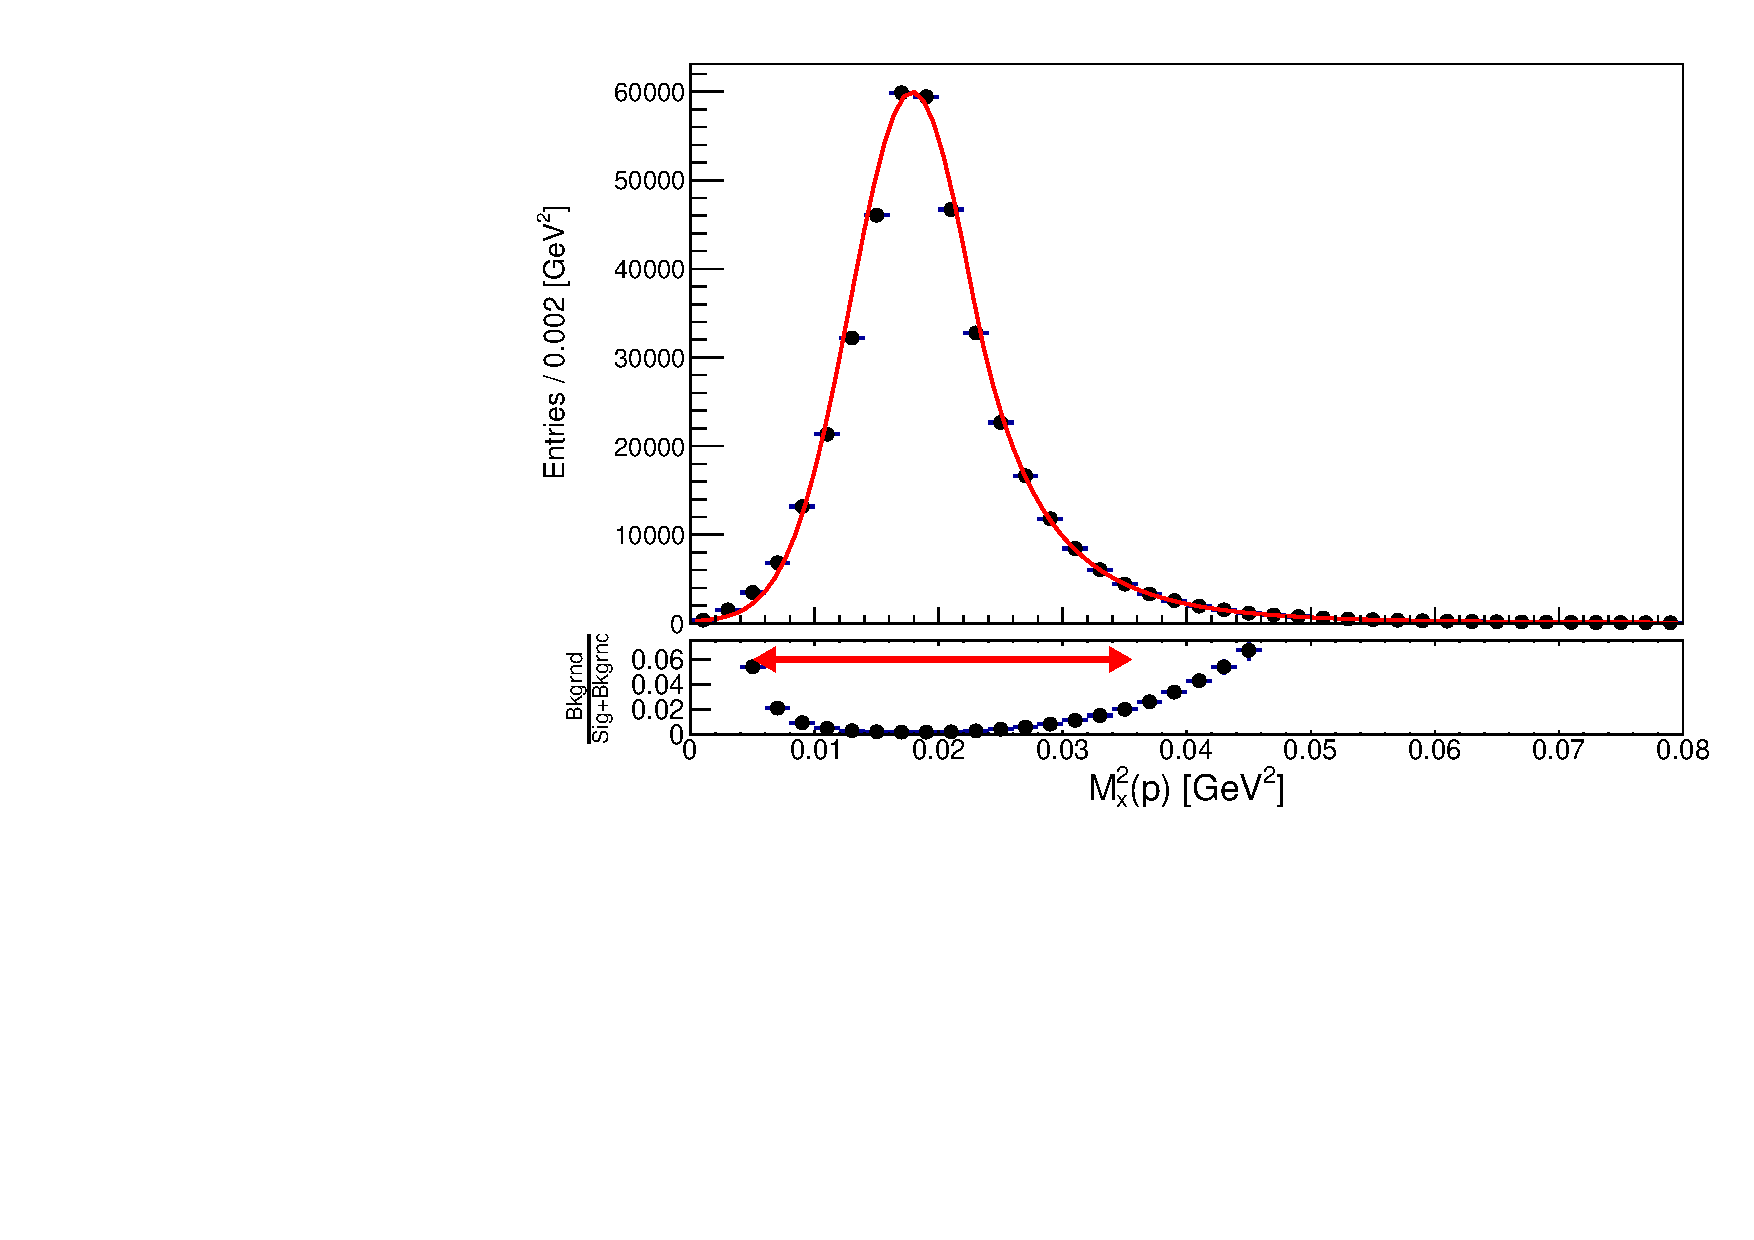
\includegraphics[height=0.35\textwidth,width=0.5\textwidth]{G12_Pi0_wBck.pdf}}

        \caption {(Color online) (top-panel) Peak of $\pi^0$ in the missing
        mass \textcolor{red}{squared} of the proton for events with $pe^+e^-(\gamma)$ in the final state.
        The red-solid line depicts the fit function (signal+background).
        (bottom-panel) Relative contributions of $\frac{\mathrm{Background}}
        {\mathrm{Signal + Background}}$. The red arrow indicates the cut
        placed on the $M_x^2(p)$ distribution to select \pizT events.}
        \label{fig:pi0_peak}
\end{figure}

The remainder of the background was attributed to $\pi^+\pi^-$
events. To reduce the background further, a comparison of the 
missing mass squared off the proton, $\mathrm{M_x^2(p) =(P_\gamma + P_p -P^{'}_p)^2}$, where $\mathrm{P's}$ are four-momenta of the incoming photon, target proton and final state proton, and the missing energy of detected system was performed, see Fig.~\ref{fig:sys}. This 
comparison revealed that the majority of $\pi^+\pi^-$ background 
has missing energy less than 75~MeV. To eliminate this background 
all events with a missing energy less than 75~MeV were removed.

The distribution of the proton missing mass squared for events with 
$pe^+e^-(\gamma)$ in the final state is shown in Fig.~\ref{fig:pi0_peak}. 
A fit was performed with the Crystal Ball function~\cite{Oreglia:1980cs,
Skwarnicki:1986xj} for the signal, plus a 3rd order polynomial function 
for the background. The total signal+background fit is shown by a red solid 
line. The fit resulted in $M_{\pi^0}^2$ = 0.0179~GeV$^2$ and the Gaussian 
$\sigma$=0.0049~GeV$^2$. To select \pizT events, an asymmetric cut, from 
the measured mean value, was placed in the range $0.0056 \le  M_x^2(p) 
\le 0.035$. This cut range can be seen as the arrow in the bottom 
panel of Fig.~\ref{fig:pi0_peak} along with the ratio of background 
events to the total number of events. As shown in Fig.~\ref{fig:pi0_peak}, 
the event selection strategy for this analysis led to a 
negligible integrated background estimated to be no more than $1.05\%$.

Overall the systematic uncertainty varied between 9\% and 12\% as a function of energy. The individual contributions came from particle efficiency, sector-to-sector efficiency, 
flux determination, missing energy cut, the kinematic fitting probabilities, 
target length, branching ratio, fiducial cut, and the z-vertex cut.
The largest contributions to the systematic uncertainties 
were the sector-to-sector (4.4 -- 7.1\%), flux determination (5.7\%),
and the cut on the 1-C pull probability (1.6 -- 6.1\%). All systematic 
uncertainties and their determinations are described in Ref.~\cite{Kunkel}.

%-----------------------------------------------------
%\textbf{Results:} 

%----------------------------------------------------
\begin{figure*}[htb!]
\centerline{
	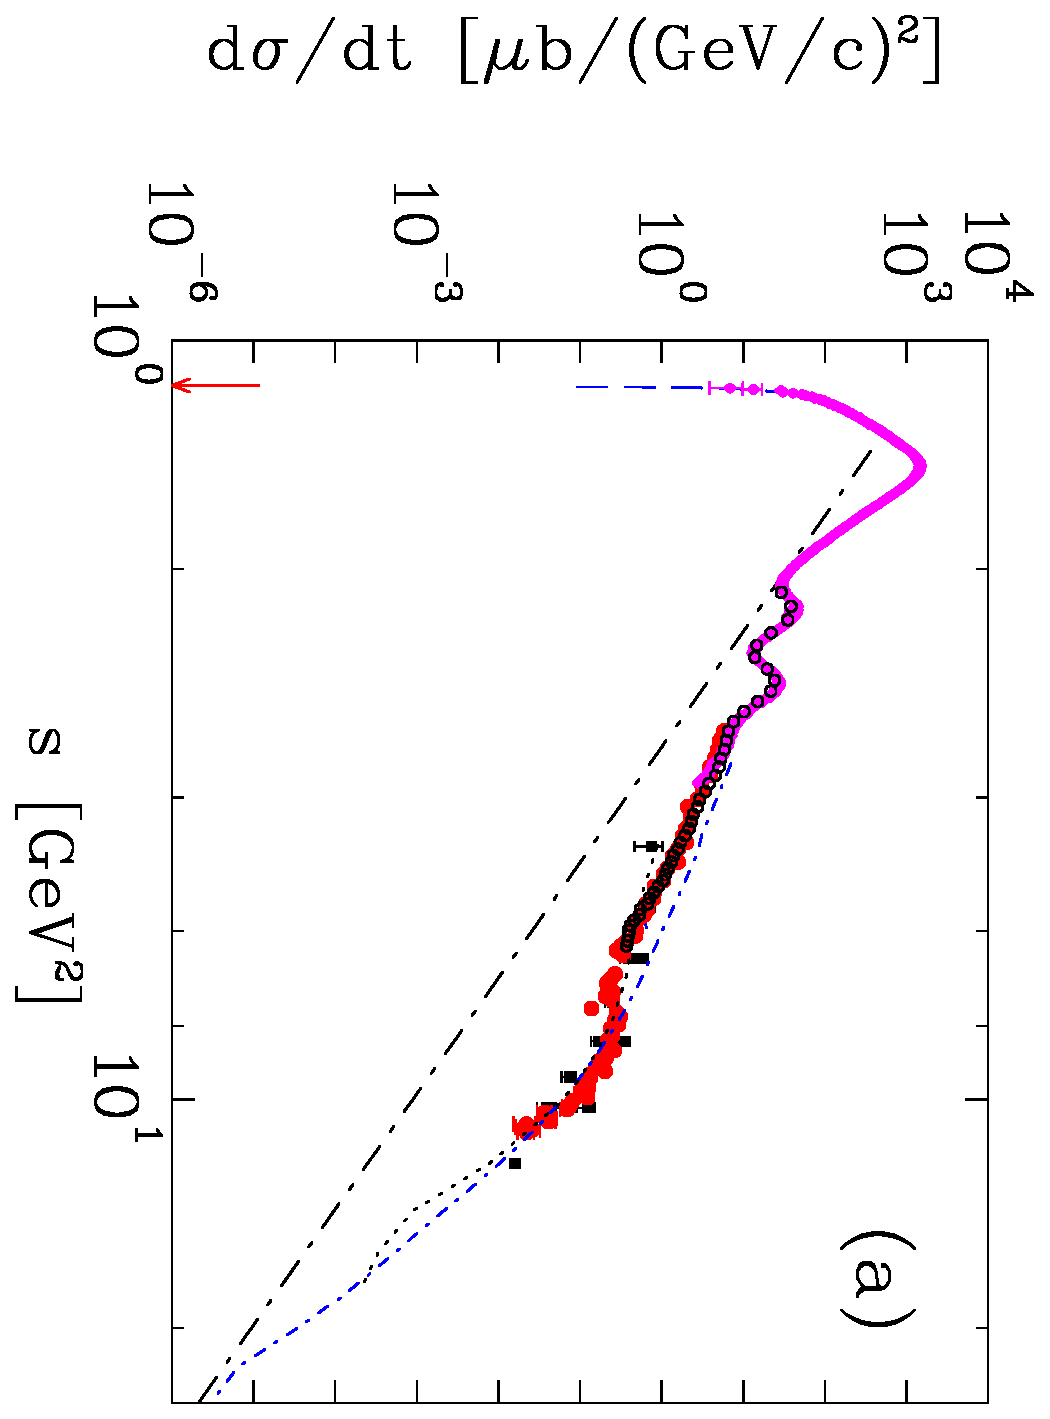
\includegraphics[height=0.4\textwidth, angle=90]{scale50.eps}\hfill%\hspace{1.5cm}
	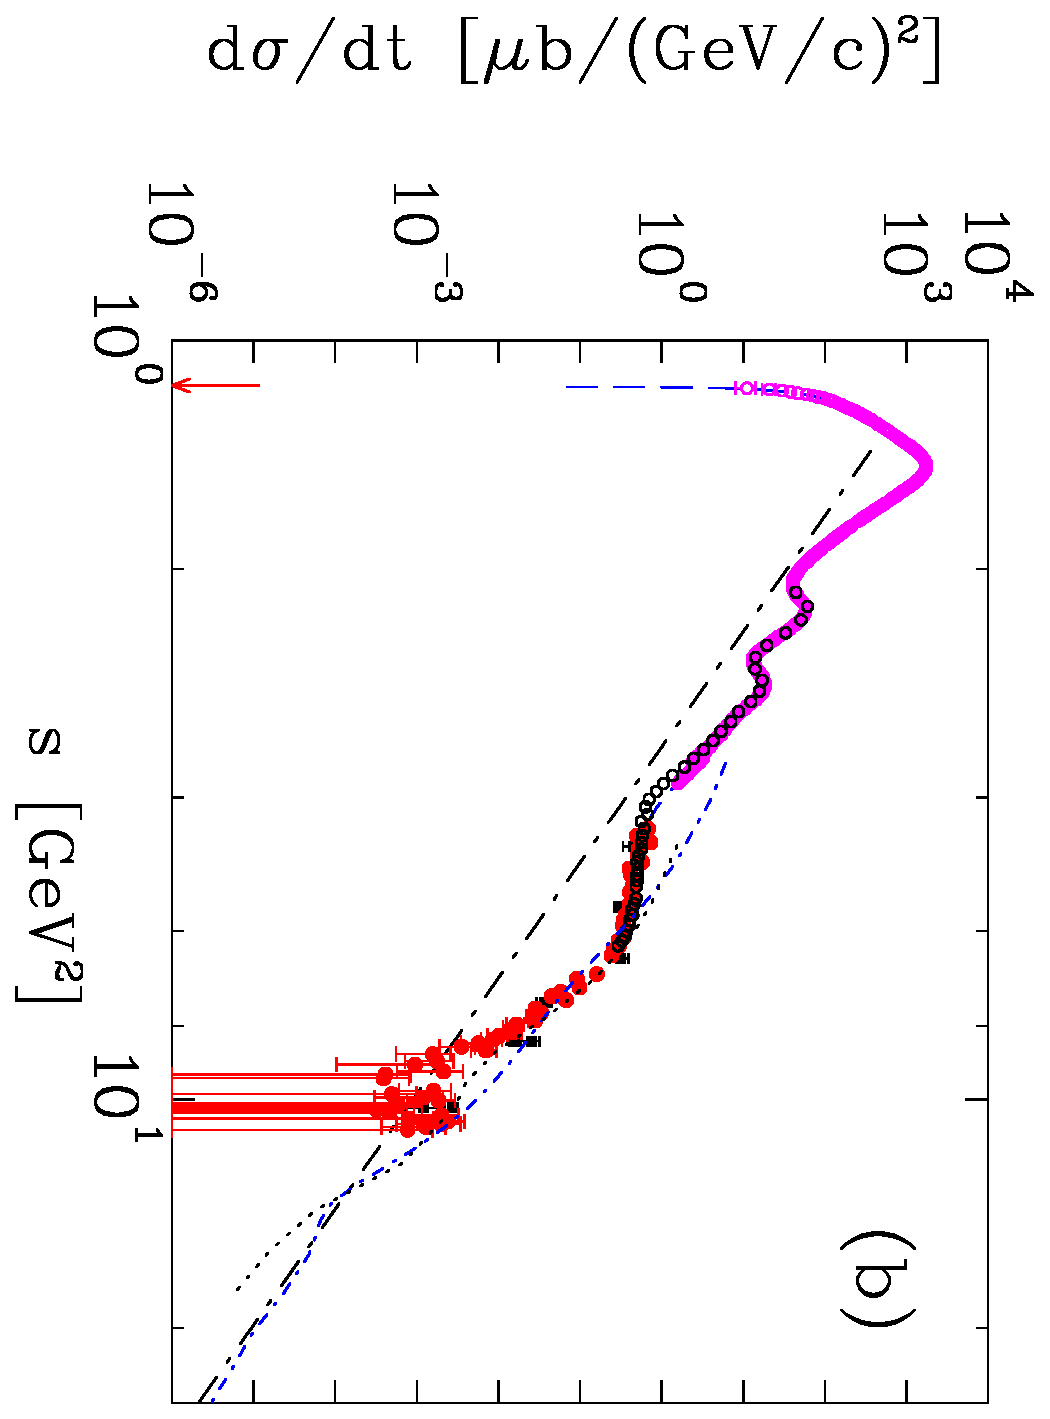
\includegraphics[height=0.4\textwidth, angle=90]{scale70.eps}}
\centerline{
        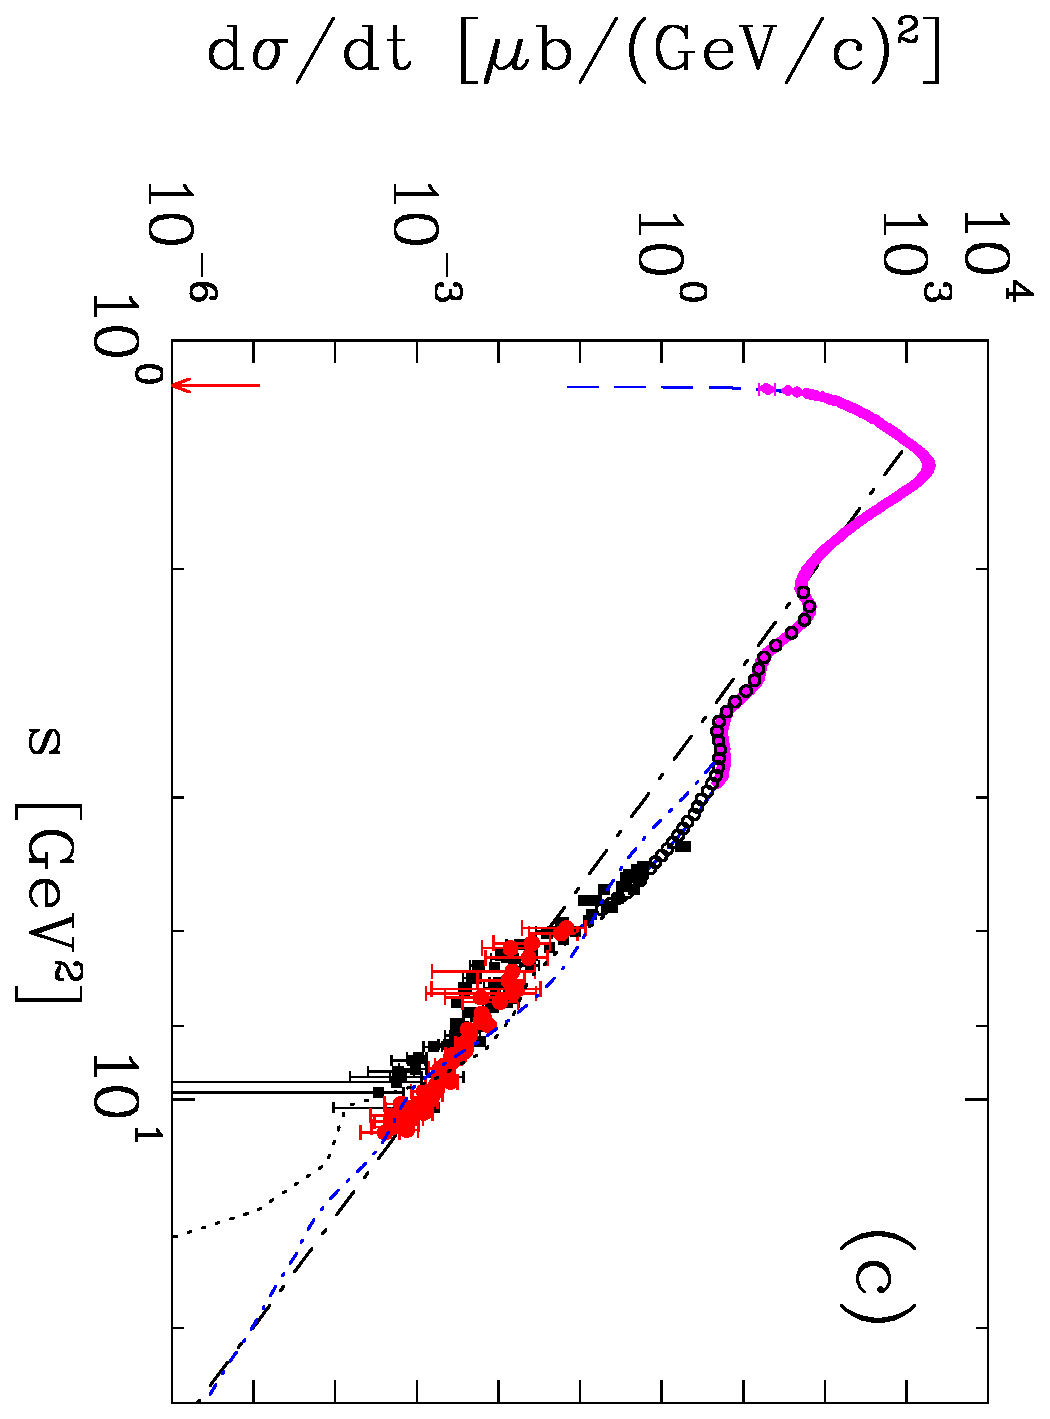
\includegraphics[height=0.4\textwidth, angle=90]{scale90.eps}\hfill%\hspace{1.5cm}
        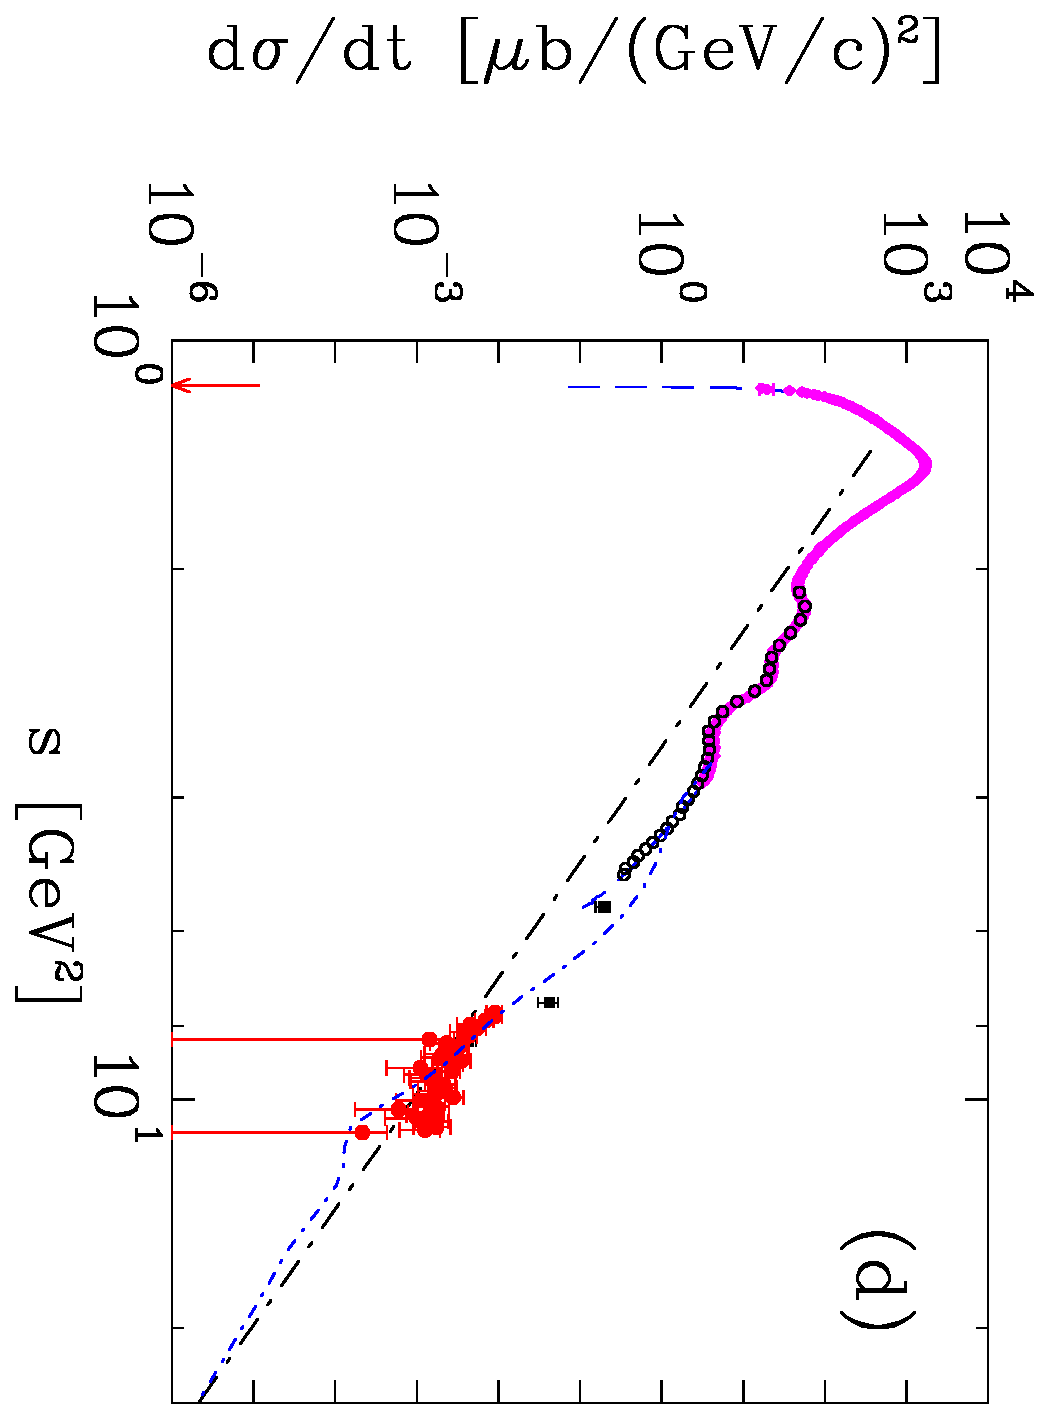
\includegraphics[height=0.4\textwidth, angle=90]{scale110.eps}}

        \caption {(Color online) Differential cross section of 
        	$\gamma p\rightarrow\pi^0p$ d$\sigma$/dt(s) at polar angles 
        	of (a) 50$^\circ$, (b) 70$^\circ$, 
        	(c) 90$^\circ$, and (d) 
        	110$^\circ$ in the c.m. frame as a function of c.m. energy 
        	squared, $s$. The red filled circles are the current $g12$ 
        	CLAS data. The recent tagged data are from previous 
        	CLAS Collaboration 
        	measurements~\protect\cite{Dugger:2007bt} (black open 
        	circles) and the A2 Collaboration at 
        	MAMI~\protect\cite{Adlarson:2015byy} 
        	(magenta open diamonds with crosses)\textcolor{red}{, while} black  filled 
        	squares are data from old bremsstrahlung measurements above 
        	E = 2~GeV~\protect\cite{brem}. Plotted uncertainties are 
        	statistical.  
        	The blue dashed line corresponds to the SAID PWA 
        	PR15 solution (no new CLAS $g12$ data are used 
        	for the fit)~\protect\cite{Adlarson:2015byy}.  Black dot-dashed 
        	lines are plotted as the best fit result of the power function $s^{-n}$, with n = 6.89$\pm$0.26, for the spectrum at 
        	90$^\circ$. Pion production threshold is shown as a vertical 
        	red arrow. Regge results~\protect\cite{Goldstein:1973xn,
        		Laget:2005be} are given by black dotted and blue dash-dotted, 
        	respectively.} \label{fig:scaling}
\end{figure*}
%-----------------------------------------------------
\textcolor{red}{
As it was mentioned above there are two subprocesses that may led to the same final state $\pi^0 \rightarrow e^+e^-\gamma$. Both subprocesses
were simulated in the Monte Carlo with their corresponding branching ratios and used to obtain cross sections from experimentally observed yield of neutral pions.}

The new CLAS high statistics cross sections, presented here, for
$\gamma p\rightarrow\pi^0p$ are compared in Figs.~\ref{fig:scaling}
and \ref{fig:t_data} with data from previous CLAS
measurements~\cite{Dugger:2007bt}, and bremsstrahlung DESY, Cambridge
Electron Accelerator (CEA), and SLAC, and Electron Synchrotron at
Cornell Univ. experiments~\cite{brem} and lower c.m. energy MAMI A2 measurements~\protect\cite{Adlarson:2015byy}. The overall agreement is good,
particularly with the previous CLAS data.
%-----------------------------------------------------
\begin{figure*}[htb!]
\centerline{
        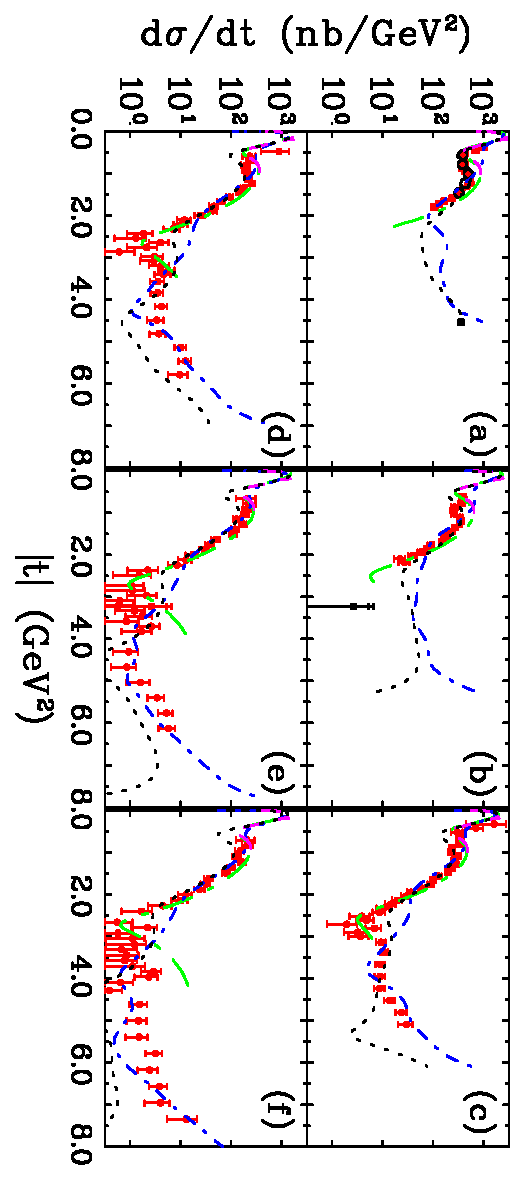
\includegraphics[width=3in, angle=90]{dsdt.eps}}

        \caption {(Color online) Samples of the $\pi^0$ photoproduction 
	cross section, $d\sigma/dt(|t|)$, off the proton versus $|t|$ 
	above ``resonance" regime.  
	(a) E = 2825~MeV and W = 2490~MeV, 
	(b) E = 3225~MeV and W = 2635~MeV,
	(c) E = 3675~MeV and W = 2790~MeV, 
	(d) E = 4125~MeV and W = 2940~MeV,
	(e) E = 4575~MeV and W = 3080~MeV, and
	(f) E = 4875~MeV and W = 3170~MeV.
	Tagged experimental data are from the current CLAS $g12$ (red 
	filled circles) and a previous CLAS 
	measurement~\protect\cite{Dugger:2007bt} (black open circles). 
	The plotted points from previously published bremsstrahlung 
	experimental data above E = 2~GeV~\protect\cite{brem} (black 
	filled squares) are those data points within $\Delta E = 
	\pm$3~MeV of the photon energy in the laboratory system 
	indicated on each panel. The uncertainties plotted are only 
	statistical. 
	Regge results~\protect\cite{Goldstein:1973xn,Laget:2005be,
	Mathieu:2015eia,Donnachie:2015jaa} are given by black dotted, 
	blue short dash-dotted, green long dash-dotted, and magenta 
	long dashed lines, respectively.} 
	\label{fig:t_data}
\end{figure*}

%-----------------------------------------------------
%\FloatBarrier

At higher energies (above $s\sim$ 6~GeV$^2$) and large c.m. angles 
($\theta\geq$ 90$^\circ$), the results are consistent with 
the $s^{-7}$ scaling, at fixed $t/s$, as expected from the 
constituent counting rule~\cite{Brodsky:1973kr}. 
The black dash-dotted line at 90$^\circ$ (Fig.~\ref{fig:scaling}) 
is a result of the fit of new CLAS $g12$ data only, performed with a 
power function $\sim s^{-n}$, leading to n = 6.89$\pm$0.26.  
Structures observed at 50$^\circ$ and 70$^\circ$ up to 
s$\sim$10~GeV$^2$ indicate that the constituent 
counting rule requires higher energies and higher $|t|$ before it 
can provide a complete description.

%-----------------------------------------------------
%\textbf{Comparison to Phenomenological Models:} 

In Figs.~\ref{fig:t_data} and \ref{fig:kroll}, the 
$d\sigma/dt(|t|)$ results are shown along with predictions from 
Regge pole and cut~\cite{Goldstein:1973xn,Laget:2005be,
Mathieu:2015eia,Donnachie:2015jaa} models and the 
handbag~\cite{Huang:2000kd} model. 

Below $|t|\sim$0.6~GeV$^2$ there is a small difference between 
different Regge approaches.  Overall, the Regge approximation 
becomes less applicable below E = 3~GeV (Fig.~\ref{fig:t_data}).  
Note that some small dips start to appear around $|t| = 0.6$~GeV$^2$
~($\cos\theta = 0.6-0.8$) where the Regge models predict a dip.  
The dip at about $|t|\sim$5~GeV$^2$ is best modeled by~\cite{Mathieu:2015eia}. Prior to this measurement there was no indication of these dips
Note that the Regge amplitudes impose non-negligible constraints when continued down to the 
``resonance" region.
Our data show another visible dip above E = 3.6~GeV at around $|t|\sim$2.6~GeV$^2$ and possible manifestation of another``possible new structure'' around $|t|\sim$5~GeV$^2$ for E $>$ 4.1~GeV, where the Regge models~\cite{Goldstein:1973xn,
Laget:2005be,Donnachie:2015jaa} predict wrong signature zeroes, 
this is where the Regge trajectories cross negative even integers. 
For the dominant vector meson Regge poles, these dips should appear 
at approximately $-t=0.6, \, 3.0, \, 5.0$~GeV$^2$,  which agrees 
with the data.  The description of the $\pi^0$ photoproduction 
cross sections at largest $|t|$ requires improving the 
Regge model by including additional exchange mechanisms.

Fig.~\ref{fig:kroll} shows that the new CLAS data are orders of 
magnitude higher than the handbag model prediction~\cite{Huang:2000kd} for $\pi^0$ 
photoproduction below $s$ = 11~GeV$^2$ (double 
solid line).
%------------------------------------------------------
%\begin{figure}[htb!]
\begin{figure}
\centerline{
        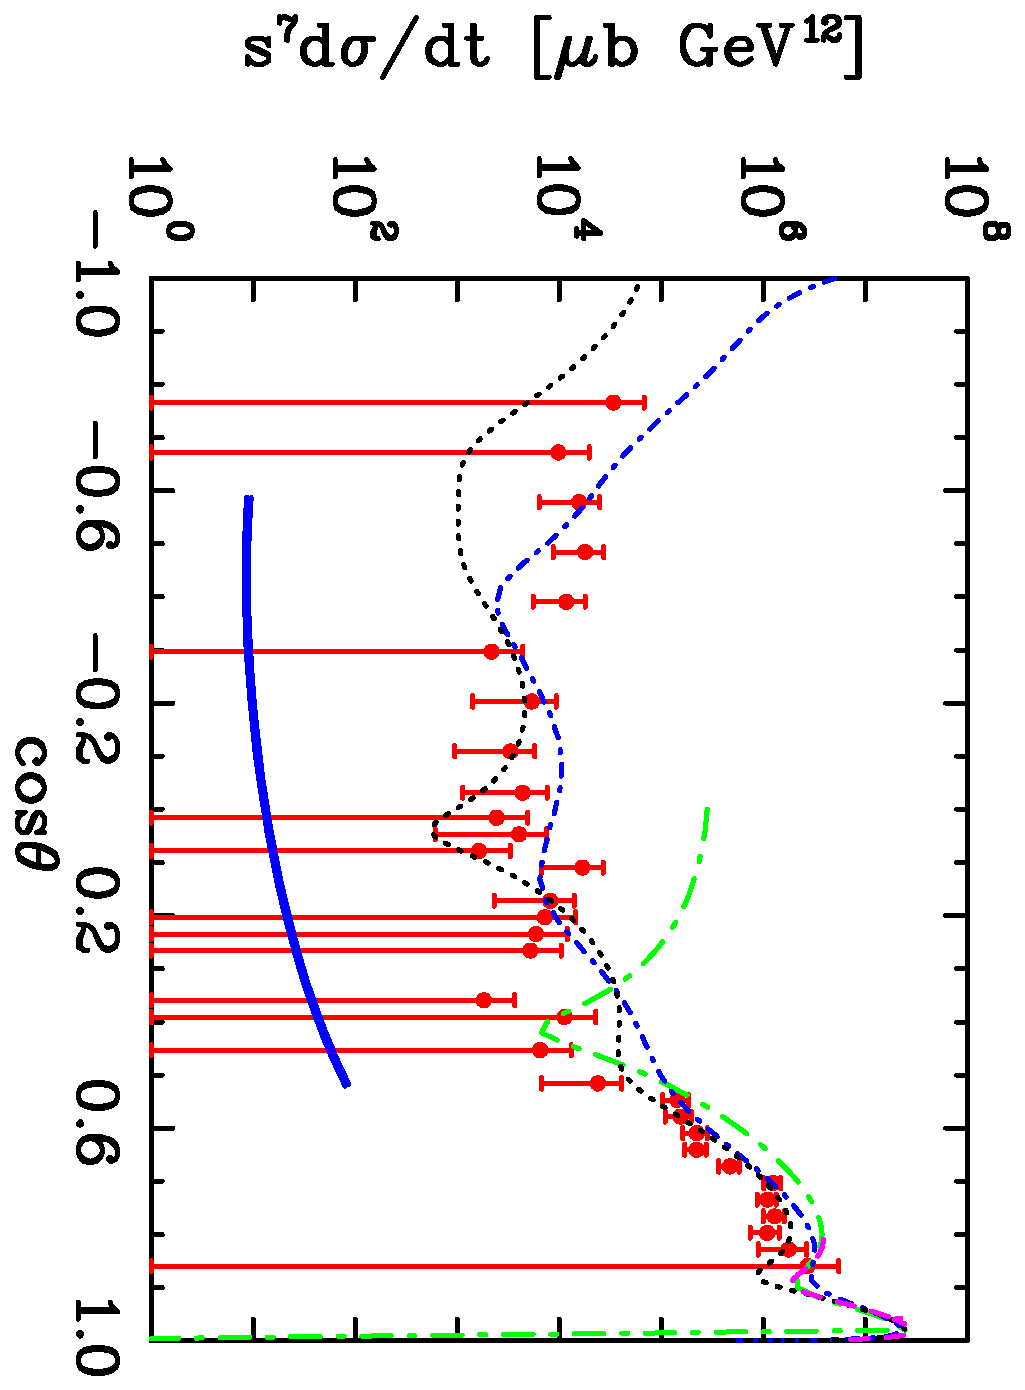
\includegraphics[width=2.5in, angle=90]{kroll.eps}}

        \caption {(Color online) Differential cross section 
	of $\pi^0$ photoproduction. The CLAS experimental data 
	at $s$ = 11~GeV$^2$ are from the current experiment (red 
	filled circles). The theoretical curves for the Regge 
	fits are the same as in Fig.~\protect\ref{fig:t_data} 
	and the handbag model by Kroll~\textit{et 
	al.}~\protect\cite{Huang:2000kd} (blue double solid 
	line).} \label{fig:kroll}
\end{figure}

%-----------------------------------------------------
%\FloatBarrier
%-----------------------------------------------------
%\textbf{Conclusions:} 

Through the experiments described above, an extensive and precise 
data set (2030 data points) on the differential cross section for 
$\pi^0$ photoproduction from the proton has been obtained 
for the first time, except for a few points from previous measurements, 
over the range of $1.81~\leq W\leq 3.33$~GeV. 

In this experiment a novel approach was employed based on Dalitz decay 
mode. Although this decay mode has a branching fraction of only about 1\%, 
the enhanced event trigger selectivity enabled the figure of merit to be 
sufficiently high in order to extend the existing world measurements into 
an essentially unmeasured {\it terra incognita} domain.

Measurements were 
performed in the reaction $\gamma p\rightarrow pe^+e^-X(\gamma)$ 
using a tagged photon beam spanning the energy interval covered 
by ``resonance" and ``Regge" regimes.
The measurements obtained here have been compared to existing 
data. The overall agreement is good, while the data provided 
here quadrupled the world bremsstrahlung database above E = 
2~GeV and covered the previous reported energies with finer 
resolution. By comparing this new and greatly expanded data set 
to the predictions of several phenomenological models, the 
present data were found to support the Regge pole model and the 
constituent counting rule while disfavoring the handbag approach.
  
%---------------------------------------------
%\FloatBarrier
%\textbf{Acknowledgements:}  
The results presented in this paper form part of the 
PhD dissertation of Michael~C.~Kunkel.  We thank Stanley Brodsky, 
Alexander Donnachie, Peter Kroll, Jean-Marc Laget, Vincent Mathieu, 
and Anatoly Radyushkin for discussions of our measurements. We 
would like to acknowledge the outstanding efforts of the staff of 
the Accelerator and the Physics Divisions at Jefferson Lab that 
made the experiment possible.  This work was supported in part by 
the Italian Istituto Nazionale di Fisica Nucleare, the French 
Centre National de la Recherche Scientifique and Commissariat \`a 
l'Energie Atomique, the United Kingdom's Science and Technology 
Facilities Council (STFC), the U.~S. DOE and NSF, and the National Research Foundation of Korea. The Southeastern Universities 
Research Association (SURA) operates the Thomas Jefferson National 
Accelerator Facility for the US DOE under contract DEAC05--84ER40150.

%-----------------------------------------------------------
\begin{thebibliography}{99}

\bibitem{Ader:1967tqj} 
  J.~P.~Ader, M.~Capdeville, and P.~Salin,
  %``A Regge pole model fit of pion and K meson photoproduction,''
  Nucl.\ Phys.\ B {\bf 3}, 407 (1967).
  %doi:10.1016/0550-3213(67)90011-9
  %%CITATION = doi:10.1016/0550-3213(67)90011-9;%%
  %30 citations counted in INSPIRE as of 19 Sep 2017

\bibitem{Armenian:1974xd} 
  H.~K.~Armenian, G.~R.~Goldstein, J.~P.~Rutherfoord, and D.~L.~Weaver,
  %``Semilocal Duality in pi0 Photoproduction,''
  Phys.\ Rev.\ D {\bf 12}, 1278 (1975).
  %doi:10.1103/PhysRevD.12.1278
  %%CITATION = doi:10.1103/PhysRevD.12.1278;%%
  %1 citations counted in INSPIRE as of 19 Sep 2017

\bibitem{Brodsky:1973kr} 
  S.~J.~Brodsky and G.~R.~Farrar,
  %``Scaling Laws at Large Transverse Momentum,''
  Phys.\ Rev.\ Lett.\  {\bf 31}, 1153 (1973).
  %doi:10.1103/PhysRevLett.31.1153
  %%CITATION = doi:10.1103/PhysRevLett.31.1153;%%
  %1719 citations counted in INSPIRE as of 19 Sep 2017

\bibitem{Goldstein:1973xn} 
  G.~R.~Goldstein and J.~F.~Owens,
  %``Pi0 photoproduction in a weak-regge-cut model,''
  Phys.\ Rev.\ D {\bf 7}, 865 (1973).
  %doi:10.1103/PhysRevD.7.865
  %%CITATION = doi:10.1103/PhysRevD.7.865;%%
  %31 citations counted in INSPIRE as of 19 Sep 2017

\bibitem{AlGhoul:2017nbp} 
  H.~Al Ghoul {\it et al.} [GlueX Collaboration],
  %``Measurement of the beam asymmetry $\Sigma$ for $\pi^0$ and $\eta$ photoproduction on the proton at $E_\gamma = 9$ GeV,''
  Phys.\ Rev.\ C {\bf 95}, no. 4, 042201 (2017).
  %doi:10.1103/PhysRevC.95.042201
  %[arXiv:1701.08123 [nucl-ex]].
  %%CITATION = doi:10.1103/PhysRevC.95.042201;%%
  %8 citations counted in INSPIRE as of 19 Sep 2017

\bibitem{Mathieu:2015eia} 
  V.~Mathieu, G.~Fox, and A.~P.~Szczepaniak,
  %``Neutral Pion Photoproduction in a Regge Model,''
  Phys.\ Rev.\ D {\bf 92}, no. 7, 074013 (2015);
  %doi:10.1103/PhysRevD.92.074013
  %[arXiv:1505.02321 [hep-ph]].
  %%CITATION = doi:10.1103/PhysRevD.92.074013;%%
  %15 citations counted in INSPIRE as of 19 Sep 2017
%\cite{Nys:2016vjz}
%\bibitem{Nys:2016vjz} 
  J.~Nys {\it et al.} [JPAC Collaboration],
  %``Finite-energy sum rules in eta photoproduction off a nucleon,''
  Phys.\ Rev.\ D {\bf 95}, no. 3, 034014 (2017).
  %doi:10.1103/PhysRevD.95.034014
  %[arXiv:1611.04658 [hep-ph]].
  %%CITATION = doi:10.1103/PhysRevD.95.034014;%%
  %10 citations counted in INSPIRE as of 19 Sep 2017

\bibitem{Kashevarov:2017vyl} 
  V.~L.~Kashevarov, M.~Ostrick and L.~Tiator,
  %``Regge phenomenology in $\pi^0$ and $\eta$ photoproduction,''
  Phys.\ Rev.\ C {\bf 96}, 035207 (2017).
  %doi:10.1103/PhysRevC.96.035207
  %[arXiv:1706.07376 [hep-ph]].
  %%CITATION = doi:10.1103/PhysRevC.96.035207;%%
  %1 citations counted in INSPIRE as of 21 Sep 2017

\bibitem{Donnachie:2015jaa} 
  A.~Donnachie and Y.~S.~Kalashnikova,
  %``Photoproduction of $a_0(980)$ and $f_0(980)$,''
  Phys.\ Rev.\ C {\bf 93}, no. 2, 025203 (2016).
  %doi:10.1103/PhysRevC.93.025203
  %[arXiv:1507.07408 [hep-ph]].
  %%CITATION = doi:10.1103/PhysRevC.93.025203;%%
  %12 citations counted in INSPIRE as of 19 Sep 2017

\bibitem{Laget:2005be}
  J.~M.~Laget,
  %``The Primakoff effect on a proton target,''
  Phys.\ Rev.\ C {\bf 72}, 022202 (2005);
  %doi:10.1103/PhysRevC.72.022202
  %[hep-ph/0502233].
  %%CITATION = doi:10.1103/PhysRevC.72.022202;%%
  %20 citations counted in INSPIRE as of 19 Sep 2017
%\cite{Guidal:1997hy}
%\bibitem{Guidal:1997hy}
  M.~Guidal, J.~M.~Laget, and M.~Vanderhaeghen,
  %``Pion and kaon photoproduction at high-energies: Forward and intermediate angles,''
  Nucl.\ Phys.\ A {\bf 627}, 645 (1997).
  %doi:10.1016/S0375-9474(97)00612-X
  %%CITATION = doi:10.1016/S0375-9474(97)00612-X;%%
  %242 citations counted in INSPIRE as of 19 Sep 2017

\bibitem{Huang:2000kd} 
  H.~W.~Huang and P.~Kroll,
  %``Large momentum transfer electroproduction of mesons,''
  Eur.\ Phys.\ J.\ C {\bf 17}, 423 (2000);
  %doi:10.1007/s100520000500
  %[hep-ph/0005318].
  %%CITATION = doi:10.1007/s100520000500;%%
  %59 citations counted in INSPIRE as of 19 Sep 2017
%\cite{Huang:2003jd}
%\bibitem{Huang:2003jd} 
  H.~W.~Huang, R.~Jakob, P.~Kroll, and K.~Passek-Kumericki,
  %``Signatures of the handbag mechanism in wide angle photoproduction of pseudoscalar mesons,''
  Eur.\ Phys.\ J.\ C {\bf 33}, 91 (2004);
  %doi:10.1140/epjc/s2003-01576-6
  %[hep-ph/0309071].
  %%CITATION = doi:10.1140/epjc/s2003-01576-6;%%
  %31 citations counted in INSPIRE as of 19 Sep 2017
%\cite{Diehl:2013xca}
%\bibitem{Diehl:2013xca} 
  M.~Diehl and P.~Kroll,
  %``Nucleon form factors, generalized parton distributions and quark angular momentum,''
  Eur.\ Phys.\ J.\ C {\bf 73}, no. 4, 2397 (2013).
  %doi:10.1140/epjc/s10052-013-2397-7
  %[arXiv:1302.4604 [hep-ph]].
  %%CITATION = doi:10.1140/epjc/s10052-013-2397-7;%%
  %73 citations counted in INSPIRE as of 19 Sep 2017

\bibitem{Ji:1996nm} 
  X.~D.~Ji,
  %``Deeply virtual Compton scattering,''
  Phys.\ Rev.\ D {\bf 55}, 7114 (1997);
  %doi:10.1103/PhysRevD.55.7114
  %[hep-ph/9609381].
  %%CITATION = doi:10.1103/PhysRevD.55.7114;%%
  %1048 citations counted in INSPIRE as of 19 Sep 2017
%\cite{Radyushkin:1996nd}
%\bibitem{Radyushkin:1996nd} 
  A.~V.~Radyushkin,
  %``Scaling limit of deeply virtual Compton scattering,''
  Phys.\ Lett.\ B {\bf 380}, 417 (1996);
  %doi:10.1016/0370-2693(96)00528-X
  %[hep-ph/9604317].
  %%CITATION = doi:10.1016/0370-2693(96)00528-X;%%
  %611 citations counted in INSPIRE as of 19 Sep 2017
%\cite{Radyushkin:1997ki}
%\bibitem{Radyushkin:1997ki} 
  A.~V.~Radyushkin,
  %``Nonforward parton distributions,''
  Phys.\ Rev.\ D {\bf 56}, 5524 (1997);
  %doi:10.1103/PhysRevD.56.5524
  %[hep-ph/9704207].
  %%CITATION = doi:10.1103/PhysRevD.56.5524;%%
  %1006 citations counted in INSPIRE as of 19 Sep 2017
%\bibitem{Mueller:1998fv} 
  D.~M\"uller, D.~Robaschik, B.~Geyer, F.-M.~Dittes, and J.~Horejsi,
  %``Wave functions, evolution equations and evolution kernels from light ray operators of QCD,''
  Fortsch.\ Phys.\  {\bf 42}, 101 (1994).
  %doi:10.1002/prop.2190420202
  %[hep-ph/9812448].
  %%CITATION = doi:10.1002/prop.2190420202;%%
  %1038 citations counted in INSPIRE as of 20 Sep 2017

\bibitem{Amarian:2000vx} 
  M.~Amarian {\it et al.} [HERMES Collaboration],
  %``Deeply virtual Compton scattering at HERMES,''
  DESY-HERMES-00-47;
  %%CITATION = DESY-HERMES-00-47;%%
  %1 citations counted in INSPIRE as of 20 Sep 2017
  AIP\ Conf.\ Proc.\ \textbf{570}, 428 (2001), Proceedings of the \textit{14th 
  International Spin Physics Symposium} (SPIN 2000), Osaka, Japan, Oct. 2000, 
  edited by K.~Hatanaka, T.~Nakano, K.~Imai, and H.~Ejiri.

\bibitem{Anderson:1976ph} 
  R.~L.~Anderson, D.~Gustavson, D.~Ritson, G.~A.~Weitsch, H.~J.~Halpern, R.~Prepost, D.~H.~Tompkins, and D.~E.~Wiser,
  %``Measurements of Exclusive Photoproduction Processes at Large Values of t and u from 4-GeV to 7.5-GeV,''
  Phys.\ Rev.\ D {\bf 14}, 679 (1976).
  %doi:10.1103/PhysRevD.14.679
  %%CITATION = doi:10.1103/PhysRevD.14.679;%%
  %102 citations counted in INSPIRE as of 19 Sep 2017

\bibitem{Jenkins:1995bk} 
  D.~A.~Jenkins and I.~I.~Strakovsky,
  %``Nucleon helicity in pion photoproduction,''
  Phys.\ Rev.\ C {\bf 52}, 3499 (1995).
  %doi:10.1103/PhysRevC.52.3499
  %[hep-ph/9509289].
  %%CITATION = doi:10.1103/PhysRevC.52.3499;%%
  %2 citations counted in INSPIRE as of 19 Sep 2017

\bibitem{Zhu:2002su} 
  L.~Y.~Zhu {\it et al.} [Jefferson Lab Hall A Collaboration],
  %``Cross-section measurement of charged pion photoproduction from hydrogen and deuterium,''
  Phys.\ Rev.\ Lett.\  {\bf 91}, 022003 (2003).
  %doi:10.1103/PhysRevLett.91.022003
  %[nucl-ex/0211009].
  %%CITATION = doi:10.1103/PhysRevLett.91.022003;%%
  %54 citations counted in INSPIRE as of 19 Sep 2017

\bibitem{Chen:2009sda} 
  W.~Chen {\it et al.},
  %``A Measurement of the differential cross section for the reaction gamma n ---> pi- p from deuterium,''
  Phys.\ Rev.\ Lett.\  {\bf 103}, 012301 (2009).
  %doi:10.1103/PhysRevLett.103.012301
  %[arXiv:0903.1260 [nucl-ex]].
  %%CITATION = doi:10.1103/PhysRevLett.103.012301;%%
  %33 citations counted in INSPIRE as of 19 Sep 2017

\bibitem{Kong:2015yzn} 
  K.~J.~Kong, T.~K.~Choi, and B.~G.~Yu,
  %``Role of $\omega$-meson exchange in scaling of the $\gamma p\rightarrow\pi^0 p$ process from a Regge-type model with resonances,''
  Phys.\ Rev.\ C {\bf 94}, no. 2, 025202 (2016).
  %doi:10.1103/PhysRevC.94.025202
  %[arXiv:1512.00238 [nucl-th]].
  %%CITATION = doi:10.1103/PhysRevC.94.025202;%%
  %1 citations counted in INSPIRE as of 19 Sep 2017

\bibitem{brem} The Durham HEP Reaction Data Databases (UK) (Durham 
	HepData): http://durpdg.dur.ac.uk/hepdata/reac.html .

\bibitem{Dugger:2007bt} 
  M.~Dugger {\it et al.},
  %``pi0 photoproduction on the proton for photon energies from 0.675 to 2.875-GeV,''
  Phys.\ Rev.\ C {\bf 76}, 025211 (2007).
  %doi:10.1103/PhysRevC.76.025211
  %[arXiv:0705.0816 [hep-ex]].
  %%CITATION = doi:10.1103/PhysRevC.76.025211;%%
  %82 citations counted in INSPIRE as of 19 Sep 2017
\bibitem{Kroll:2017hym} 
P.~Kroll,
%``The GPD $\tilde {H}$ and spin correlations in wide-angle Compton scattering,''
Eur.\ Phys.\ J.\ A {\bf 53}, no. 6, 130 (2017) and references therein.
%doi:10.1140/epja/i2017-12326-2
%[arXiv:1703.05000 [hep-ph]].
%%CITATION = doi:10.1140/epja/i2017-12326-2;%%
%1 citations counted in INSPIRE as of 19 Sep 2017

\bibitem{g12} G12 experimental group, CLAS-NOTE 2017 - 002, 2017 
	\url{https://misportal.jlab.org/ul/Physics/Hall-B/clas/viewFile.cfm/2017-002.pdf?documentId=756}.

\bibitem{Kunkel} M.~C.~Kunkel,  CLAS-NOTE 2017 - 005, 2017 
	\url{https://misportal.jlab.org/ul/Physics/Hall-B/clas/viewFile.cfm/2017-005.pdf?documentId=767}.

\bibitem{PLUTO} I.~Frohlich {\it et al.}, 
	PoS ACAT {\bf }, 076 (2007) [arXiv:0708.2382 [nucl-ex]].

\bibitem{Oreglia:1980cs} 
  M.~Oreglia,
  %``A Study of the Reactions $\psi^\prime \rightarrow\gamma \gamma \psi$,''
  SLAC Stanford - SLAC-236 (80,REC.APR. 81) 226p; 
  %214 citations counted in INSPIRE as of 19 Sep 2017
  Ph.~D.~Thesis, SLAC, 1980.

\bibitem{Skwarnicki:1986xj} 
  T.~Skwarnicki,
  %``A study of the radiative CASCADE transitions between the Upsilon-Prime and Upsilon resonances,''
  DESY-F31-86-02, DESY-F-31-86-02;
  %%CITATION = DESY-F31-86-02, DESY-F-31-86-02;%%
  %519 citations counted in INSPIRE as of 19 Sep 2017
  Ph.~D.~Thesis, Inst.\ Nucl.\ Phys.\ Cracow, Poland, 1986.

\bibitem{Adlarson:2015byy} 
  P.~Adlarson {\it et al.} [A2 Collaboration at MAMI],
  %``Measurement of $.^0$ photoproduction on the proton at MAMI C,''
  Phys.\ Rev.\ C {\bf 92}, no. 2, 024617 (2015).
  %doi:10.1103/PhysRevC.92.024617
  %[arXiv:1506.08849 [hep-ex]].
  %%CITATION = doi:10.1103/PhysRevC.92.024617;%%
  %13 citations counted in INSPIRE as of 19 Sep 2017
\end{thebibliography}
%---------------------------------------------------------------------
\end{document}
